\documentclass[12pt]{article}
\usepackage{amsmath,amssymb}
\usepackage{amsfonts}
\usepackage{graphicx}	
\usepackage{float}
\usepackage{physics}
\usepackage{multirow}
\usepackage{subcaption}
%\usepackage{nicematrix}
\usepackage{cite}
\usepackage{caption}
\usepackage{blkarray,booktabs,bigstrut}
\usepackage{hyperref}
\usepackage{xcolor}\hypersetup{colorlinks=true,linkcolor=blue,pdftitle={Kondo with Magnetic field}}
\usepackage[margin=0.8in,top=1.0in,bottom=1.4in]{geometry}
\title{Kondo with Magnetic field}
\author{Debraj Debata\\[1ex] 
\small 20IP014}

\date{ 2022-23}

\newcommand{\matindex}[1]{\mbox{\scriptsize#1}}

\newcommand{\bigzero}{\mbox{\normalfont\Large\bfseries 0}}
\newcommand{\rvline}{\hspace*{-\arraycolsep}\vline\hspace*{-\arraycolsep}}








\begin{document}
\textbf{$J$ Renormalisation}:
\begin{align*}
\Delta J & = - \frac{J^2}{2}\Big[\frac{1}{w-\frac{D}{2} + \frac{J}{8} + t_{\perp}} + \frac{1}{w-\frac{D}{2} + \frac{J}{8} - t_{\perp}} \Big] \\ 
& =  \frac{J^2}{2}\Big[\frac{1}{d_0 + t_{\perp}} + \frac{1}{d_0 - t_{\perp}} \Big] \\
\Delta J & = J^2 \frac{d_0}{d_0^2 - t_{\perp}^2}
\end{align*}
We have taken $d_0 = -w +\frac{D}{2} -\frac{J}{8}$.\\
\textbf{For MCK type Case}:
\begin{align*}
\Delta J & = \frac{J^2}{2 (d_0 - t_{\perp})}(1 + \frac{d_0 - t_{\perp}}{2d_0}) \\
& = \frac{J^2}{2 (d_0 - t_{\perp})}(\frac{3}{2} - \frac{t_{\perp}}{2d_0})
\end{align*}
Here $d_0 - t_{\perp}$ is small compare to $d_0$ and $\Delta J$ will change sign due to denominator $(d_0 - t_{\perp})$ before the first bracket starts.

\textbf{For e-SIAM type case}:
\begin{align*}
\Delta J = - J^2 \frac{d_0}{t_{\perp}^2} (1 + \frac{d_0^2}{t_{\perp}^2})
\end{align*}
Here $d_0$ is small compare to $t_{\perp}$ and $\Delta J$ will change sign due to numerator $d_0$ before the first bracket starts.\\
\textbf{$V$ Renormalisation}:
\begin{align*}
\Delta V & = \frac{3VJ}{8} \Big[\frac{d_0}{d_0^2 - t_{\perp}^2} + \frac{d_0 - \frac{U}{2}}{(d_0 - \frac{U}{2})^2 - t_{\perp}^2} \Big] \\
& = \frac{3VJ}{8} \Big[\frac{\Delta J}{J^2} + \frac{d_0 - \frac{U}{2}}{(d_0 - \frac{U}{2})^2 - t_{\perp}^2} \Big]
\end{align*}\\
\textbf{U Renormalisation}:
\begin{align*}
\Delta U & = 4 V^2 \Big[\frac{d_0 + \frac{J}{8} + \frac{U}{2}}{(d_0 + \frac{J}{8} + \frac{U}{2})^2 - t_{\perp}^2}  -\frac{d_0 - \frac{U}{2}}{(d_0 - \frac{U}{2})^2 - t_{\perp}^2} \Big] + J^2 \frac{d_0}{d_0^2 - t_{\perp}^2} \\
& =  4 V^2 \Big[\frac{d_0 + \frac{J}{8} + \frac{U}{2}}{(d_0 + \frac{J}{8} + \frac{U}{2})^2 - t_{\perp}^2}  -\frac{8 \Delta V}{3VJ} + \frac{\Delta J}{J^2} \Big] + \Delta J \\
& = 4 V^2 \frac{d_0 + \frac{J}{8} + \frac{U}{2}}{(d_0 + \frac{J}{8} + \frac{U}{2})^2 - t_{\perp}^2} - \frac{32 V}{3J} \Delta V + (1 + 4 \frac{V^2}{J^2} )\Delta J
\end{align*}


\begin{figure}[!ht]
    \centering
    \includegraphics[scale=0.4]{D0=10.png}
    \caption{D0=10}
\end{figure}

\begin{figure}[!ht]
    \centering
    \includegraphics[scale=0.4]{D0=1000.png}
    \caption{D0=1000}
\end{figure}

\newpage



\begin{figure}[!ht]
    \centering
    \includegraphics[scale=0.3]{like-e-SIAM-tD=0.9.png}
    \includegraphics[scale=0.3]{like-e-SIAM-tD=1.png}
    \includegraphics[scale=0.3]{like-e-SIAM-tD=1.1.png}
    \caption{With $U_b$ like e-SIAM }
\end{figure}

\begin{figure}[!ht]
    \centering
    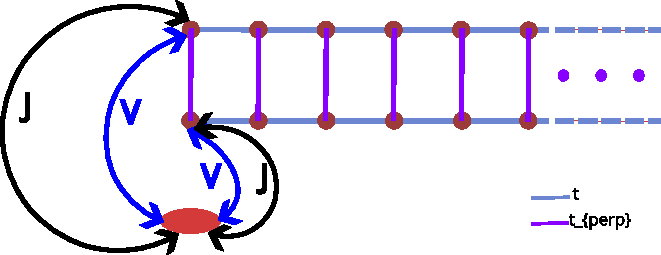
\includegraphics[scale=1.5]{3-orbital-figure.pdf}
\end{figure}

\end{document}